\documentclass[conference]{IEEEtran}
\IEEEoverridecommandlockouts
% The preceding line is only needed to identify funding in the first footnote. If that is unneeded, please comment it out.
\usepackage{cite}
\usepackage{amsmath,amssymb,amsfonts}
\usepackage{algorithmic}
\usepackage{graphicx}
\usepackage{textcomp}
\usepackage{xcolor}
\usepackage[brazilian]{babel}
\usepackage[utf8]{inputenc}
\usepackage[T1]{fontenc}
\usepackage{listings}
\usepackage{listings-golang}
\usepackage{color}
\usepackage{float}
\usepackage{multirow}
\usepackage{hyperref}

\definecolor{dkgreen}{rgb}{0,0.6,0}
\definecolor{gray}{rgb}{0.5,0.5,0.5}
\definecolor{mauve}{rgb}{0.58,0,0.82}

\lstset{frame=tb,
  language=Golang,
  aboveskip=3mm,
  belowskip=3mm,
  showstringspaces=false,
  columns=flexible,
  basicstyle={\small\ttfamily},
  numbers=none,
  numberstyle=\tiny\color{gray},
  keywordstyle=\color{blue},
  commentstyle=\color{dkgreen},
  stringstyle=\color{mauve},
  breaklines=true,
  breakatwhitespace=true,
  tabsize=3
}
\lstset{language=Golang}
\def\BibTeX{{\rm B\kern-.05em{\sc i\kern-.025em b}\kern-.08em
    T\kern-.1667em\lower.7ex\hbox{E}\kern-.125emX}}
\begin{document}

\title{Relatório da Atividade 2: \\ Exclusão Mútua\\
}

\author{\IEEEauthorblockN{Isabelle Ferreira de Oliveira}
\IEEEauthorblockA{\textit{CES-27 - Engenharia da Computação 2020} \\
\textit{Instituto Tecnológico de Aeronáutica (ITA)}\\
São José dos Campos, Brasil \\
isabelle.ferreira3000@gmail.com}
}

\maketitle

\begin{abstract}
Esse relatório documenta a implementação do algoritmo de Ricart-Agrawala, um algoritmo de exclusão mútua para sistemas distribuídos.
\end{abstract}

\begin{IEEEkeywords}
Algoritmo de Ricart-Agrawala, exclusão mútua, Relógio lógico vetorial, sistemas distribuídos
\end{IEEEkeywords}

\section{Implementação}
	
	A implementação do recurso compartilhado se tratou principalmente da utilização do código disponibilizado no roteiro do laboratório. Dentro do loop principal, foi colocada a função de servidor, cuja implementação era simplesmente imprimir na tela qualquer mensagem recebida pela porta :10001.
	
	Abaixo encontra-se os códigods da função main() e da função doServerJob().
	
\begin{lstlisting}
func main() {
	Address, err := net.ResolveUDPAddr("udp", ":10001")
	Connection, err = net.ListenUDP("udp", Address)
	defer Connection.Close()

	for {
		doServerJob()
	}
}
\end{lstlisting}

\begin{lstlisting}
func doServerJob() {
	buf := make([]byte, 1024)

	n, _, err := Connection.ReadFromUDP(buf)
	err = json.Unmarshal(buf[:n], &messageReceived)

	fmt.Println(messageReceived.Text)
}
\end{lstlisting}

	A mensagem recebida era da forma de struct, com os atributos de id do processo que enviou a mensagem, o relógio lógico do processo que enviou a mensagem e, por fim, o texto a ser impresso no terminal.

	Vale ressaltar também que, para esse código e todos os outros dessa atividade, sempre após a setagem da variável \textit{err}, referente a um possível erro advindo de algumas funções, também era chamada a função CheckError(err), que imprime o erro e interrompe o processo caso houvesse algum erro.

	Na main(), primeiramente são iniciadas as conexões de servidores e clientes, a partir da chamada de initConnections(). Nessa função, também é iniciado o relógio lógico desse processo em questão, além de serem setados seu ID, e as portas de todos os processos. 
	
	Após isso, é iniciada uma thread para ler as entradas do usuário a partir da função readInput().
	
	Em seguida, é iniciado o loop de fazer o trabalho de servidor (ou seja, atualiza-se o relógio lógico caso chegue uma mensagem de outro processo, por meio da thread doServerJob()) e fica-se esperando uma mensagem do usuário no canal criado \textit{ch}.
	
	Ao se receber esse input do usuário, atualiza-se o relógio lógico e, a partir daí, duas ações podem ser tomadas a depender do conteúdo da entrada: 
	
\begin{itemize}
\item faz-se o trabalho de cliente (enviando uma mensagem a um outro processo por meio da thread doClientJob()) caso a entrada seja o ID de outro processo;
\item ou apenas imprime-se o valor atual do relógio lógico caso a entrada seja o próprio ID desse processo.
\end{itemize}
	
	Abaixo, segue-se o código dessa função initConnections().
	
\begin{lstlisting}
func initConnections() {
	nPorts = len(os.Args) - 2

	// my process
	logicalClock = 0
	auxMyID, err := strconv.Atoi(os.Args[1])
	myID = auxMyID
	myPort = os.Args[myID+1]

	// Server
	ServerAddr, err := net.ResolveUDPAddr("udp", myPort)
	aux, err := net.ListenUDP("udp", ServerAddr)
	ServConn = aux

	// Clients
	for i := 0; i < nPorts; i++ {
		aPort := os.Args[i+2]
		
		ServerAddr, err := net.ResolveUDPAddr("udp","127.0.0.1" + aPort)
		LocalAddr, err := net.ResolveUDPAddr("udp", "127.0.0.1:0")
		auxConn, err := net.DialUDP("udp", LocalAddr, ServerAddr)
		AllConn = append(AllConn, auxConn)
	}
}
\end{lstlisting}

	Vale ressaltar também que, para esse código e todos os outros dessa atividade, sempre após a setagem da variável \textit{err}, referente a um possível erro advindo de algumas funções, também era chamada a função CheckError(err), que imprime o erro e interrompe o processo caso houvesse algum erro.
	
	Essas chamadas de funções foram suprimidas do relatório a fim de simplificar a apresentação dos códigos, e por entender-se que não se trata da ideia principal dos códigos desenvolvidos.
	
	A função readInput() segue bem semelhante àquela apresenta na Dica 3 do roteiro, com a diferença de aceitar um canal de inteiro ao invés de um canal de string. Assim, a função é capaz de ler o ID que o usuário digitar.
	
	Já a função doServerJob(), apresentada abaixo, também segue bem semelhante à apresentada na função main() do código do servidor fornecido na Dica 1. A diferença está na retirada do loop \textit{for} e do fechamento da conexão, uma vez que essas etapas se equivalem aos apresentados na main() da atividade (função já apresentada acima). Outra diferença também é a impressão do relógio lógico recebido por mensagem e, em seguida, a impressão do valor atualizado. Segue abaixo o código descrito.

\begin{lstlisting}
func doServerJob() {
	buf := make([]byte, 1024)

	n, _, err := ServConn.ReadFromUDP(buf)

	aux := string(buf[0:n])
	otherLogicalClock, err := strconv.Atoi(aux)
	fmt.Println("Received", otherLogicalClock)
	
	// updating logical clock
	logicalClock = max(otherLogicalClock, logicalClock) + 1
	fmt.Println("logicalClock atualizado:", logicalClock)
}
\end{lstlisting}

	Por fim, a função doClientJob() também seguiu de forma semelhante ao código apresentado na função main() do código do cliente fornecido na Dica 1. As alterações também foram semelhantes: retirouse o loop \textit{for} e o fechamento da conexão. Além diso, o conteúdo da mensagem a ser enviada foi alterado para o relógio lógico atual do processo em questão. Segue abaixo o código descrito.

\begin{lstlisting}
func doClientJob(otherProcessID int, logicalClock int) {
	otherProcess := otherProcessID - 1

	msg := strconv.Itoa(logicalClock)
	buf := []byte(msg)

	_,err := AllConn[otherProcess].Write(buf)

	time.Sleep(time.Second * 1)
}
\end{lstlisting}

	A segunda etapa se tratou da implementação da simulação para o Relógio Lógico Vetorial, segundo o algoritmo descrito nos slides da aula e conforme o solicitado no roteiro da atividade. Essa implementação foi feita de forma bastante análoga à da Tarefa 1.
	
	As principais alterações na implementação foram:
\begin{itemize}
\item mudança do logicalClock de inteiro para uma \textit{struct} com o ID do processo atual e um vetor com os clocks de todos os processos;
\item alteração das mensagens recebidas e enviadas (de inteiros para \textit{jsons} contendo as \textit{structs});
\item alteração na lógica de atualização do vetor de clocks.
\end{itemize}

	O impacto dessas mudanças nas funções no código desenvolvido na Tarefa 2 em relação a Tarefa 1 foram:
	
\begin{itemize}
\item em initConnections(), a iniciação do logicalClock se trata de setar o atributo myId e criar o vetor de clocks da struct com valores iniciais zero;
\item as mensagens (structs) trocadas entre processos foram encapsuladas na forma de json a partir da função json.Marshal() e desencapsuladas com a função json.Unmarshal();
\item ao se receber a struct logicalClock de outro processo, (além de incrementar o clock referente ao processo atual) os valores de clocks eram atualizados para o máximo entre o clock armazenado e o clock recém recebido.
\end{itemize}

Como as principais alterações foram pequenas e já foram descritas acima, não se considerou necessário colocar nesse relatório as partes referentes do código da Tarefa 2. Caso seja necessário, pode-se também consultar o código enviado como anexo a essa atividade. 

\section{Resultados e Conclusões} \label{results}

\subsection{Tarefa 1}

	A implementação mostrou-se correta, uma vez que os resultados dos testes e das simulações se mostraram condizentes com o esperado.
	
	O primeiro teste executado foi apresentado na Figura \ref{tarefa1-testeslide}, e se tratava do exemplo apresentado nos slides da aula. Eram três processos ($P_1$, $P_2$ e $P_3$), e os acontecimentos se deram da seguinte maneira:
	
\begin{itemize}
\item $P_1$ realizou seu primeiro evento, incrementando seu relógio lógico para 1;
\item $P_3$ realizou seu primeiro evento, incrementando seu relógio lógico para 1;
\item $P_1$ mandou uma mensagem para $P_2$, incrementando seus relógios lógicos para 2 e 3, respectivamente;
\item $P_2$ mandou uma mensagem para $P_3$, incrementando seus relógios lógicos para 4 e 5, respectivamente.
\end{itemize}

	Como esses resultados, conforme na Figura \ref{tarefa1-testeslide}, foram exatamente os esperados de acordo com os slides da aula, tem-se que esse teste foi satisfatório.
	
%\begin{figure}[H]
%\centering
%\centerline{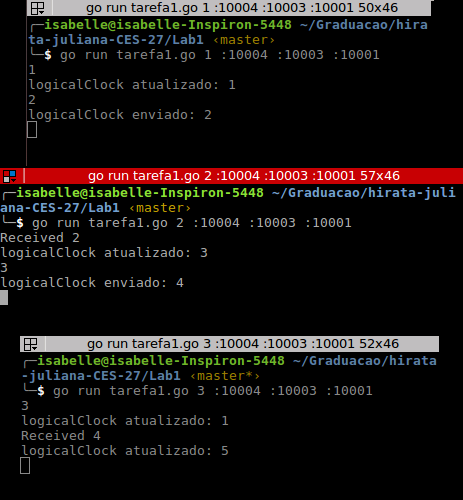
\includegraphics[scale=0.45]{imagens/tarefa1-testeslide.png}}
%\caption{Exemplo do funcionamento da Tarefa 1 para 3 processos.}.
%\label{tarefa1-testeslide}
%\end{figure}
	
	Outro teste executado foi o apresentado nas Figuras \ref{tarefa1-testecriado-1} e \ref{tarefa1-testecriado-2}. Essas duas figuras apresentam o mesmo teste, dessa vez para quatro processos, sendo a Figura \ref{tarefa1-testecriado-1} referente aos processos 1 e 3, e a Figura \ref{tarefa1-testecriado-2} aos processos 2 e 4. Os eventos aconteceram da seguinte maneira:
	
\begin{itemize}
\item $P_1$ realizou seus três primeiros eventos, incrementando seu relógio lógico para 3;
\item $P_2$ realizou seu primeiro evento, incrementando seu relógio lógico para 1;
\item $P_4$ mandou uma mensagem para $P_1$, incrementando seus relógios lógicos para 1 e 4, respectivamente;
\item $P_4$ realizou cinco eventos, incrementando seu relógio lógico para 6;
\item $P_4$ mandou uma mensagem para $P_1$, incrementando seus relógios lógicos para 7 e 8, respectivamente;
\item $P_2$ mandou uma mensagem para $P_3$, incrementando seus relógios lógicos para 2 e 3, respectivamente;
\item $P_2$ mandou uma mensagem para $P_1$, incrementando seus relógios lógicos para 3 e 9, respectivamente;
\item $P_2$ mandou uma mensagem para $P_4$, incrementando seus relógios lógicos para 4 e 8, respectivamente;
\item $P_2$ realizou um evento, incrementando seu relógio lógico para 5;
\item $P_2$ mandou uma mensagem para $P_3$, incrementando seus relógios lógicos para 6 e 7, respectivamente;
\item $P_3$ realizou três eventos, incrementando seu relógio lógico para 10;
\item $P_3$ mandou uma mensagem para $P_1$, incrementando seus relógios lógicos para 11 e 12, respectivamente.
\end{itemize}

%\begin{figure}[H]
%\centering
%\centerline{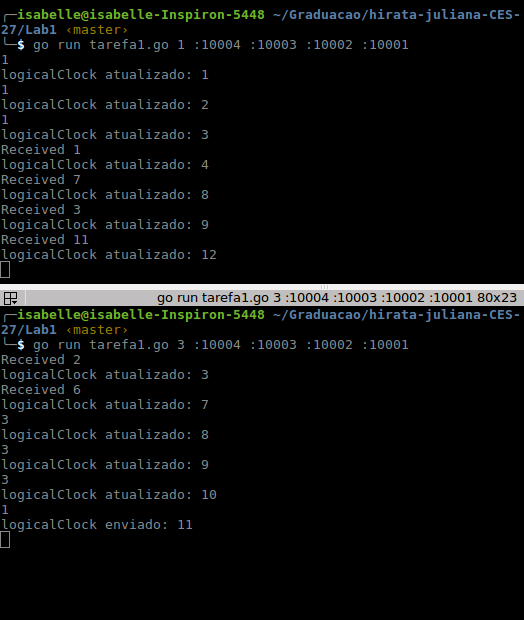
\includegraphics[scale=0.4]{imagens/tarefa1-testecriado-1.png}}
%\caption{Exemplo do funcionamento da Tarefa 1 para 4 processos. Tela dos processos 1 e 3.}.
%\label{tarefa1-testecriado-1}
%\end{figure}

%\begin{figure}[H]
%\centering
%\centerline{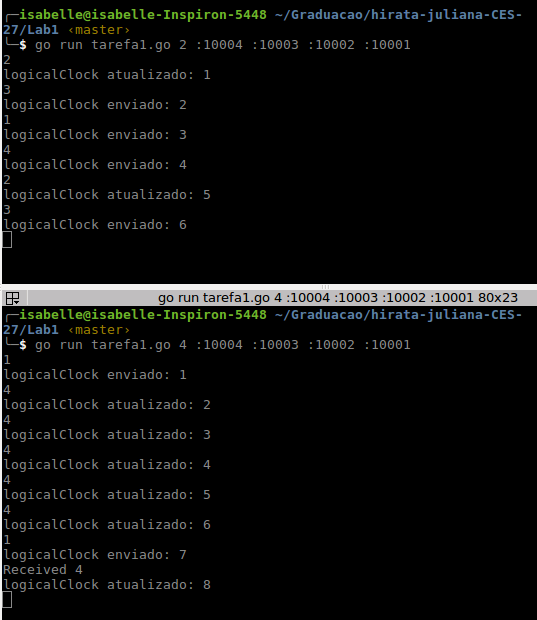
\includegraphics[scale=0.4]{imagens/tarefa1-testecriado-2.png}}
%\caption{Exemplo do funcionamento da Tarefa 1 para 4 processos. Tela dos processos 2 e 4.}.
%\label{tarefa1-testecriado-2}
%\end{figure}

	Como esses resultados também foram condizentes com os resultados esperados, conclui-se que a implementação da Tarefa 1 foi feita corretamente.

\subsection{Tarefa 2}

	A implementação também mostrou-se correta, uma vez que os resultados dos testes e das simulações se mostraram condizentes com o esperado. Os testes foram exatamente os mesmos da Tarefa 1, com a mudança apenas do tipo de relógio lógico estava sendo enviado como mensagem.
	
	O primeiro teste executado foi apresentado nas Figuras \ref{tarefa2-testeslide-1} e \ref{tarefa2-testeslide-2}, e se tratava do exemplo apresentado nos slides da aula. Eram três processos ($P_1$, $P_2$ e $P_3$), e os acontecimentos se deram da seguinte maneira:
	
\begin{itemize}
\item $P_1$ realizou seu primeiro evento, incrementando seu relógio lógico para (1, 0, 0);
\item $P_3$ realizou seu primeiro evento, incrementando seu relógio lógico para (0, 0, 1);
\item $P_1$ mandou uma mensagem para $P_2$, incrementando seus relógios lógicos para (2, 0, 0) e (2, 1, 0), respectivamente;
\item $P_2$ mandou uma mensagem para $P_3$, incrementando seus relógios lógicos para (2, 2, 0) e (2, 2, 2), respectivamente.
\end{itemize}

	Como esses resultados, conforme nas Figuras \ref{tarefa2-testeslide-1} e \ref{tarefa2-testeslide-2}, foram exatamente os esperados de acordo com os slides da aula, tem-se que esse teste foi satisfatório.

%\begin{figure}[H]
%\centering
%\centerline{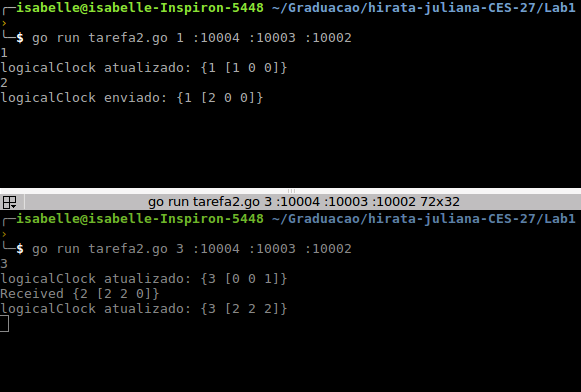
\includegraphics[scale=0.4]{imagens/tarefa2-testeslide-1.png}}
%\caption{Exemplo do funcionamento da Tarefa 2 para 3 processos. Tela dos processos 1 e 3.}.
%\label{tarefa2-testeslide-1}
%\end{figure}

%\begin{figure}[H]
%\centering
%\centerline{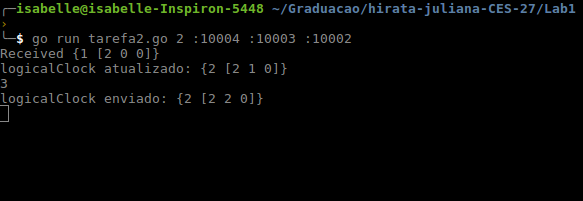
\includegraphics[scale=0.4]{imagens/tarefa2-testeslide-2.png}}
%\caption{Exemplo do funcionamento da Tarefa 2 para 3 processos. Tela do processo 2.}.
%\label{tarefa2-testeslide-2}
%\end{figure}

	Outro teste executado foi o apresentado nas Figuras \ref{tarefa1-testecriado-1} e \ref{tarefa1-testecriado-2}. Essas duas figuras apresentam o mesmo teste, dessa vez para quatro processos, sendo a Figura \ref{tarefa1-testecriado-1} referente aos processos 1 e 2, e a Figura \ref{tarefa1-testecriado-2} aos processos 3 e 4. Os eventos aconteceram da seguinte maneira:
	
\begin{itemize}
\item $P_1$ realizou seus três primeiros eventos, incrementando seu relógio lógico para (3, 0, 0, 0);
\item $P_2$ realizou seu primeiro evento, incrementando seu relógio lógico para (0, 1, 0, 0);
\item $P_4$ mandou uma mensagem para $P_1$, incrementando seus relógios lógicos para (4, 0, 0, 1) e (0, 0, 0, 1), respectivamente;
\item $P_4$ realizou cinco eventos, incrementando seu relógio lógico para (0, 0, 0, 6);
\item $P_4$ mandou uma mensagem para $P_1$, incrementando seus relógios lógicos para (5, 0, 0, 7) e (0, 0, 0, 7), respectivamente;
\item $P_2$ mandou uma mensagem para $P_3$, incrementando seus relógios lógicos para (0, 2, 0, 0) e (0, 2, 1, 0), respectivamente;
\item $P_2$ mandou uma mensagem para $P_1$, incrementando seus relógios lógicos para (0, 3, 0, 0) e (6, 3, 0, 7), respectivamente;
\item $P_2$ mandou uma mensagem para $P_4$, incrementando seus relógios lógicos para (0, 4, 0, 0) e (0, 4, 0, 8), respectivamente;
\item $P_2$ realizou um evento, incrementando seu relógio lógico para (0, 5, 0, 0);
\item $P_2$ mandou uma mensagem para $P_3$, incrementando seus relógios lógicos para (0, 6, 0, 0) e (0, 6, 2, 0), respectivamente;
\item $P_3$ realizou três eventos, incrementando seu relógio lógico para (0, 6, 5, 0);
\item $P_3$ mandou uma mensagem para $P_1$, incrementando seus relógios lógicos para (0, 6, 6, 0) e (7, 6, 6, 7), respectivamente.
\end{itemize}

%\begin{figure}[H]
%\centering
%\centerline{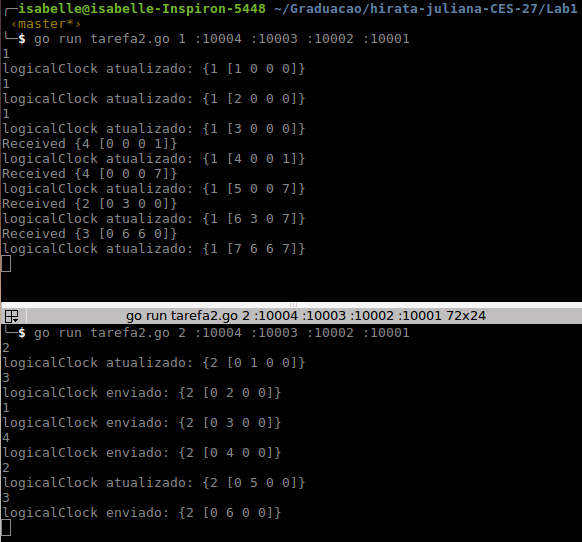
\includegraphics[scale=0.4]{imagens/tarefa2-testecriado-1.png}}
%\caption{Exemplo do funcionamento da Tarefa 2 para 4 processos. Tela dos processos 1 e 2.}.
%\label{tarefa1-testecriado-1}
%\end{figure}

%\begin{figure}[H]
%\centering
%\centerline{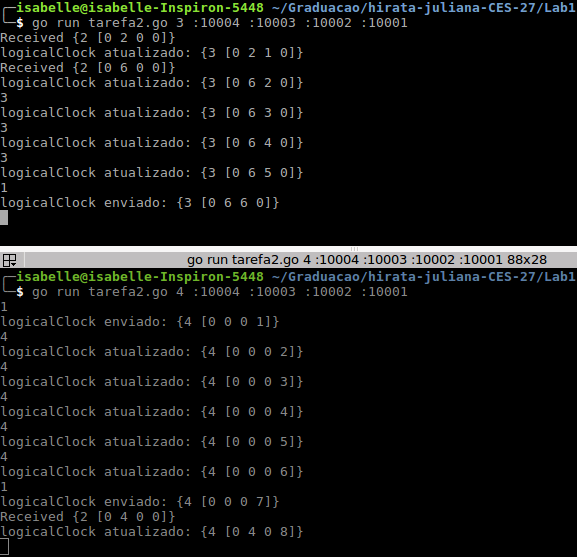
\includegraphics[scale=0.4]{imagens/tarefa2-testecriado-2.png}}
%\caption{Exemplo do funcionamento da Tarefa 2 para 4 processos. Tela dos processos 3 e 4.}.
%\label{tarefa1-testecriado-2}
%\end{figure}

	Como esses resultados também foram condizentes com os resultados esperados, conclui-se que a implementação da Tarefa 2 foi feita corretamente.
	
%\begin{thebibliography}{00}
%\bibitem{roteiro} M. Maximo, ``Roteiro: Laboratório 12 - Deep Q-Learning''. Instituto Tecnológico de Aeronáutica, Departamento de Computação. CT-213, 2019.

%\bibitem{roteiro8} M. Maximo, ``Roteiro: Laboratório 8 - Imitation Learning com Keras''. Instituto Tecnológico de Aeronáutica, Departamento de Computação. CT-213, 2019.

%\bibitem{roteiro12} M. Maximo, ``Roteiro: Laboratório 12 - Aprendizado por Reforço Livre de Modelo''. Instituto Tecnológico de Aeronáutica, Departamento de Computação. CT-213, 2019.

%\end{thebibliography}

\end{document}
